% RealFact project report, IEEE conference format (IEEEtran). Build:  make report
\documentclass[conference,a4paper]{IEEEtran}
\IEEEoverridecommandlockouts

\usepackage{cite}
\usepackage{amsmath}
\usepackage[T1]{fontenc}
\usepackage{newtxtext,newtxmath}
\usepackage{graphicx}
\usepackage{booktabs,multirow,array,tabularx}
\usepackage[table]{xcolor}
\usepackage{tikz}
\usetikzlibrary{arrows.meta,positioning,fit,calc,shapes.geometric,decorations.pathreplacing}
\usepackage{pgfplots}
\pgfplotsset{compat=1.17}
\usepgfplotslibrary{groupplots}
\usepackage{listings}
\usepackage{algorithm}
\usepackage{algpseudocode}
\usepackage[hidelinks]{hyperref}

\graphicspath{{figures/}}

\definecolor{novel}{HTML}{2F5BD3}
\definecolor{novelsoft}{HTML}{E5ECFC}
\definecolor{sup}{HTML}{1F8A57}
\definecolor{con}{HTML}{C43C3C}
\definecolor{conf}{HTML}{B7791F}
\definecolor{inkthree}{HTML}{7C818C}
\definecolor{codebg}{HTML}{F4F5F7}
\definecolor{tA}{HTML}{2F5BD3}
\definecolor{tB}{HTML}{E08A2E}

\lstset{basicstyle=\ttfamily\scriptsize,backgroundcolor=\color{codebg},frame=single,rulecolor=\color{black!15},
  keywordstyle=\color{novel}\bfseries,commentstyle=\color{inkthree}\itshape,columns=fullflexible,
  breaklines=true,showstringspaces=false,xleftmargin=2pt,xrightmargin=2pt,aboveskip=6pt,belowskip=4pt}
\newcolumntype{Y}{>{\raggedright\arraybackslash}X}
\newcolumntype{P}[1]{>{\raggedright\arraybackslash}p{#1}}
\newcommand{\yes}{\textcolor{sup}{\textbf{Yes}}}
\newcommand{\no}{\textcolor{con}{No}}
\newcommand{\partl}{\textcolor{conf}{Partial}}

\begin{document}

\title{RealFact: OpenMP-Accelerated, Independence-Aware Real-Time News Verification}

\makeatletter
\newcommand{\linebreakand}{\end{@IEEEauthorhalign}\hfill\mbox{}\par\mbox{}\hfill\begin{@IEEEauthorhalign}}
\makeatother

\author{
\IEEEauthorblockN{Adithya Shyam D}
\IEEEauthorblockA{\textit{Dept. of Information Technology}\\
\textit{NIT Karnataka, Surathkal}\\
Mangaluru, India\\
241IT005\\
adithyashyamd.241it005@nitk.edu.in}
\and
\IEEEauthorblockN{Krishna}
\IEEEauthorblockA{\textit{Dept. of Information Technology}\\
\textit{NIT Karnataka, Surathkal}\\
Mangaluru, India\\
241IT039\\
krishna.241it039@nitk.edu.in}
\linebreakand
\IEEEauthorblockN{P Suman}
\IEEEauthorblockA{\textit{Dept. of Information Technology}\\
\textit{NIT Karnataka, Surathkal}\\
Mangaluru, India\\
241IT049\\
psuman.241it049@nitk.edu.in}
\and
\IEEEauthorblockN{Saurabh}
\IEEEauthorblockA{\textit{Dept. of Information Technology}\\
\textit{NIT Karnataka, Surathkal}\\
Mangaluru, India\\
241IT072\\
saurabh.241it072@nitk.edu.in}
}

\maketitle

\begin{abstract}
Evidence-based fact-checking over live news is a large similarity-search problem, and it has a counting problem:
outlets republish the same wire story, so ten retrieved ``confirmations'' may be one report. We present RealFact, a working system that verifies a claim
against a continuously refreshed corpus of 42 RSS feeds, optionally extended by on-demand Google News and Wikipedia
search. RealFact retrieves a wide candidate pool, clusters near-duplicate copies, weights a cluster of $n$ copies as
$1+\lambda\log_2 n$ votes, and returns one of four cited verdicts: Supported, Contradicted, Conflicting Evidence or
Unverified. Three stages run as C++/OpenMP kernels. An exact top-$M$ retrieval scan reaches $4.61\times$ over a
non-OpenMP serial build at 500K articles; after an instruction-level-parallelism rewrite it becomes bandwidth-bound
at 96\,GB/s with 4 threads. A corpus-wide all-pairs duplicate detector, which is compute-bound and has a triangular
iteration space, reaches $6.92\times$ on 11 heterogeneous cores with dynamic scheduling against $4.98\times$ for
static. A block-speculative parallelisation of the sequential leader-clustering algorithm reaches $5.8\times$ with
output identical to the sequential algorithm. A 14-check suite verifies that every parallel configuration is bit-identical to the serial
build. In a controlled syndication test, naive counting flips a contested claim to Contradicted while RealFact keeps
Conflicting Evidence.
On a FEVER subset of 179 claims against 25,324 Wikipedia pages, RealFact reaches 81.0\% accuracy with settings chosen
on a disjoint tuning split.
\end{abstract}

\begin{IEEEkeywords}
fact-checking, OpenMP, parallel computing, similarity search, near-duplicate detection, natural language inference,
load balancing, roofline model
\end{IEEEkeywords}

% =====================================================================================================
\section{Introduction}

Automated fact-checking asks whether a claim is supported by the available evidence. Two weaknesses of common
approaches motivate this work. First, style-based ``fake news'' classifiers judge wording, not truth, and fail when a
false claim imitates credible reporting. Second, evidence-based systems built on benchmarks such as FEVER~\cite{fever},
LIAR~\cite{liar} and HoVer~\cite{hover} are evaluated on accuracy alone. Their latency and multicore scalability are
rarely measured, although both matter when the evidence pool is live and large.

A third problem appears when the evidence is real news. Outlets republish the same wire report, so a ranked list of
evidence can be ten copies of one story. If every copy counts as an independent confirmation, one report can outvote
several genuinely independent ones. A search engine does not solve this: it returns ranked links, often many copies of
the same story, and leaves the user to decide what they say.

\textbf{Research question.} \emph{Can large-scale, multi-source evidence retrieval for real-time news verification run
efficiently on a multicore CPU using OpenMP, without counting duplicate or syndicated reports as independent evidence?}

\textbf{Contributions.}
\begin{enumerate}
  \item An \emph{independence-aware aggregation} stage: retrieve wide, cluster near-duplicates, keep the top-$K$
  clusters, weight each by $w_c=1+\lambda\log_2 n_c$, and issue a cited four-way verdict (Section~\ref{sec:design}).
  \item Three \emph{OpenMP kernels} with deterministic, bit-exact output: an exact top-$M$ scan, a corpus-wide
  all-pairs duplicate detector, and a block-speculative parallel leader clustering (Section~\ref{sec:par}).
  \item A measurement study using course tools: strong and weak scaling, Karp--Flatt, per-thread load balance on
  heterogeneous cores, chunk-size sweeps, the roofline model, and Wilcoxon tests (Section~\ref{sec:results}).
  \item Operation on \emph{live} evidence: 42 permitted RSS feeds refreshed every 20 minutes, plus on-demand web
  search for the claim being checked, with a saved verification history.
  \item An evaluation on LIAR and on a FEVER subset with a held-out tuning split, and a web interface that runs the
  whole pipeline and shows how existing aggregation rules would judge the same evidence.
\end{enumerate}

% =====================================================================================================
\section{Background and Related Work}
\label{sec:related}

\subsection{The fact-checking framework}
Our primary reference is the survey by Guo, Schlichtkrull and Vlachos~\cite{guo2022}. It decomposes automated
fact-checking into claim detection, evidence retrieval, verdict prediction and justification production.
Fig.~\ref{fig:framework} places RealFact in that framework. Claim detection is out of scope (the user supplies the
claim); justification is partial (evidence is cited with each cluster's weight and contribution, but no free-text
explanation is generated).

\begin{figure}[!t]
\centering

\begin{tikzpicture}[
  stage/.style={draw,rounded corners=2pt,minimum width=1.85cm,minimum height=0.95cm,align=center,font=\scriptsize},
  fwin/.style={stage,fill=novelsoft,draw=novel,line width=0.8pt},
  fwout/.style={stage,dashed,draw=inkthree,fill=black!3},
  arr/.style={-{Stealth[length=1.6mm]},thick,inkthree}]
\node[fwout] (a) {\textbf{Claim}\\\textbf{detection}\\[-1pt]\tiny out of scope};
\node[fwin,right=0.22cm of a] (b) {\textbf{Evidence}\\\textbf{retrieval}\\[-1pt]\tiny\textcolor{novel}{RealFact}};
\node[fwin,right=0.22cm of b] (c) {\textbf{Verdict}\\\textbf{prediction}\\[-1pt]\tiny\textcolor{novel}{RealFact}};
\node[fwout,right=0.22cm of c] (d) {\textbf{Justifi-}\\\textbf{cation}\\[-1pt]\tiny partial};
\draw[arr] (a)--(b); \draw[arr] (b)--(c); \draw[arr] (c)--(d);
\end{tikzpicture}
\caption{The fact-checking framework of~\cite{guo2022}; RealFact covers the highlighted stages.}
\label{fig:framework}
\end{figure}

\subsection{Lessons from the survey}
Table~\ref{tab:lessons} lists the survey points that shaped the design. The most important are that verdicts should be
computed from evidence rather than claim wording; that conflicting and untrustworthy evidence is an open problem,
since most systems assume a single trustworthy source; that ``not enough information'' is a legitimate outcome; and
that benchmarks are static while real claims concern recent events.

\begin{table}[!t]
\caption{Survey lessons and RealFact's response}
\label{tab:lessons}
\centering\footnotesize
\setlength{\tabcolsep}{3pt}
\renewcommand{\arraystretch}{1.25}
\begin{tabularx}{\columnwidth}{P{0.40\columnwidth}Y}
\toprule
\textbf{Survey point (paraphrased)} & \textbf{RealFact decision}\\
\midrule
Retrieval then verdict prediction & Separate, separately timed stages; verdicts come from evidence only.\\
Claim-only datasets invite surface cues & Every verdict lists its evidence; no evidence gives \emph{Unverified}.\\
Conflicting evidence is open & \emph{Conflicting Evidence} is a verdict; syndicated copies are discounted.\\
NEI is a legitimate outcome & Sufficiency threshold $\theta$ and a relevance floor.\\
Dataset artefacts, evidence leakage & Several datasets; an exclusion mask removes a claim's own article.\\
Static snapshots vs.\ recent claims & Live RSS ingestion and on-demand web search.\\
Efficiency rarely reported & OpenMP kernels measured and checked bit-for-bit against serial.\\
\bottomrule
\end{tabularx}
\end{table}

\subsection{Existing approaches}
FEVER~\cite{fever} established retrieve-then-classify over Wikipedia with SUPPORTED/REFUTED/NOT ENOUGH INFO labels.
LIAR~\cite{liar} has 12,836 political statements on a six-point scale but no evidence documents.
FakeNewsNet~\cite{fakenewsnet} provides full articles with source URLs. HoVer~\cite{hover} extends retrieval to
multi-hop reasoning. Table~\ref{tab:compare} compares them with RealFact. None of them handles syndicated duplicates
or reports parallel performance.

\begin{table*}[!t]
\caption{Comparison with existing approaches (last row: this work)}
\label{tab:compare}
\centering\footnotesize
\setlength{\tabcolsep}{4pt}
\begin{tabularx}{\textwidth}{P{2.4cm}YP{1.7cm}YYP{1.4cm}YY}
\toprule
\textbf{System} & \textbf{Evidence} & \textbf{Up to date} & \textbf{Retrieval} & \textbf{Duplicate handling} & \textbf{Verdicts} & \textbf{Conflicting evidence} & \textbf{Parallel performance}\\
\midrule
Style classifiers & None (writing style) & --- & None & --- & Binary & \no & \no\\
LIAR baselines~\cite{liar} & Claim + metadata & Static & None & --- & 6-way & \no & \no\\
FEVER pipeline~\cite{fever} & Wikipedia & Static dump & Document + sentence top-$k$ & None & 3-way & Folded into NEI & Accuracy only\\
HoVer~\cite{hover} & Wikipedia, multi-hop & Static dump & Iterative multi-hop & None & 2--3-way & \no & Accuracy only\\
\rowcolor{novelsoft}\textbf{RealFact} & Live multi-outlet news, web search, Wikipedia & \yes{} (RSS + search) & Exact OpenMP scan, top-$M$ with $M\gg K$ & Cluster at $\tau$; $w=1+\lambda\log_2 n$ & 4-way, cited & \yes{} (first-class) & \yes{} (3 kernels, speedup, $E_p$, Karp--Flatt, Wilcoxon)\\
\bottomrule
\end{tabularx}
\end{table*}

% =====================================================================================================
\section{System Design}
\label{sec:design}

Fig.~\ref{fig:arch} shows the architecture. The \emph{index} side ingests evidence into a contiguous $N\times384$
float32 embedding matrix. The \emph{verify} side retrieves, clusters, classifies and aggregates. A separate
benchmarking arm times the kernels only, so the systems claim and the accuracy claim can fail independently.

\begin{figure*}[!t]
\centering
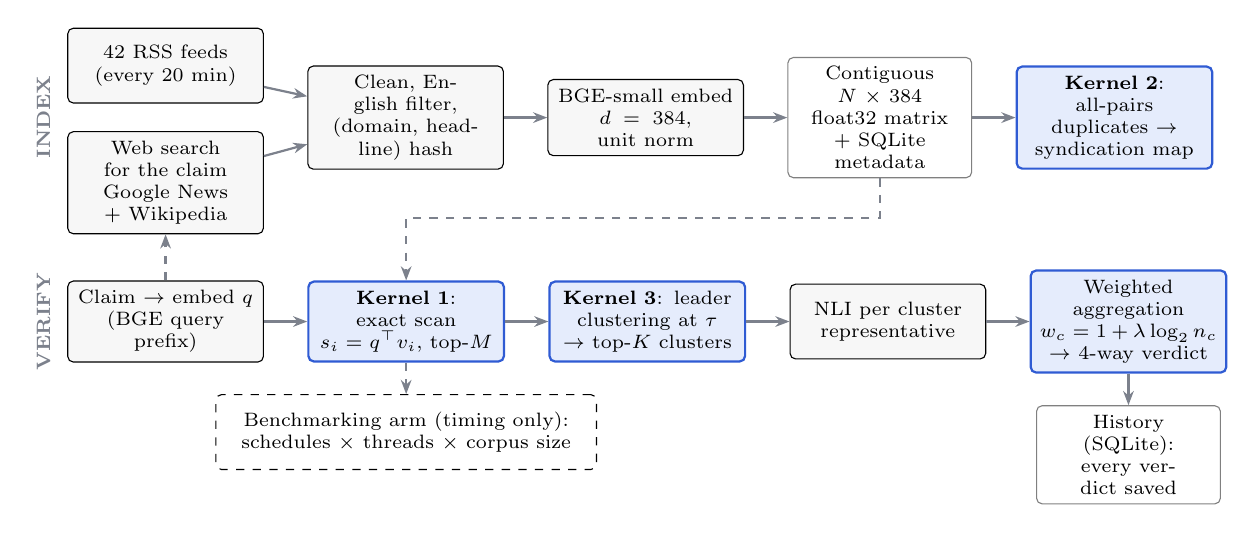
\begin{tikzpicture}[
  box/.style={draw,rounded corners=2pt,align=center,font=\scriptsize,minimum height=0.95cm,text width=2.25cm,fill=black!3},
  nov/.style={box,fill=novelsoft,draw=novel,line width=0.8pt},
  store/.style={box,fill=white,draw=black!50,text width=2.1cm},
  arr/.style={-{Stealth[length=1.8mm]},thick,inkthree},
  lab/.style={font=\scriptsize\bfseries,inkthree,anchor=west}]
\node[lab,rotate=90,anchor=center] at (-1.55,-0.65) {INDEX};
\node[box] (rss) at (0,0) {42 RSS feeds\\(every 20 min)};
\node[box,below=0.35cm of rss] (web) {Web search for the claim\\Google News + Wikipedia};
\node[box,right=0.55cm of rss,yshift=-0.66cm] (clean) {Clean, English filter,\\(domain, headline) hash};
\node[box,right=0.55cm of clean] (emb) {BGE-small embed\\$d=384$, unit norm};
\node[store,right=0.55cm of emb] (mat) {Contiguous $N\times384$\\float32 matrix\\+ SQLite metadata};
\node[nov,right=0.55cm of mat] (syn) {\textbf{Kernel 2}: all-pairs\\duplicates $\to$\\syndication map};
\draw[arr] (rss) -- (clean); \draw[arr] (web) -- (clean); \draw[arr] (clean) -- (emb); \draw[arr] (emb) -- (mat); \draw[arr] (mat) -- (syn);
\node[lab,rotate=90,anchor=center] at (-1.55,-3.25) {VERIFY};
\node[box] (claim) at (0,-3.25) {Claim $\to$ embed $q$\\(BGE query prefix)};
\node[nov,right=0.55cm of claim] (scan) {\textbf{Kernel 1}: exact scan\\$s_i=q^\top v_i$, top-$M$};
\node[nov,right=0.55cm of scan] (clu) {\textbf{Kernel 3}: leader\\clustering at $\tau$\\$\to$ top-$K$ clusters};
\node[box,right=0.55cm of clu] (nli) {NLI per cluster\\representative};
\node[nov,right=0.55cm of nli] (agg) {Weighted aggregation\\$w_c=1+\lambda\log_2 n_c$\\$\to$ 4-way verdict};
\draw[arr] (claim) -- (scan); \draw[arr] (scan) -- (clu); \draw[arr] (clu) -- (nli); \draw[arr] (nli) -- (agg);
\draw[arr,dashed] (mat.south) -- ++(0,-0.5) -| (scan.north);
\draw[arr,dashed] (claim.north) -- (web.south);
\node[store,below=0.4cm of agg] (hist) {History (SQLite):\\every verdict saved};
\draw[arr] (agg) -- (hist);
\node[box,dashed,fill=white,below=0.4cm of scan,text width=4.6cm] (bench) {Benchmarking arm (timing only): schedules $\times$ threads $\times$ corpus size};
\draw[arr,dashed] (scan.south) -- (bench.north);
\end{tikzpicture}
\caption{RealFact architecture. Blue boxes are this project's contributions; the three OpenMP kernels are numbered.}
\label{fig:arch}
\end{figure*}

\subsection{Evidence sources}
\textbf{Live RSS.} 42 permitted feeds are fetched concurrently every 20 minutes. Only the headline and lead are kept;
article pages are never scraped. HTML and boilerplate are stripped, non-English items dropped, and each item is
hashed on (source domain, normalised headline), an exact-duplicate filter applied before embedding. At the time of
writing the corpus holds 3,770 articles from 40 outlets.

\textbf{On-demand web search.} When enabled, the claim is turned into a keyword query (fact-check prefixes, a leading
auxiliary verb and punctuation are removed) and two sources are queried in parallel: up to 12 Google News RSS search
results and the lead paragraphs of up to 3 Wikipedia pages through the official MediaWiki API. New items pass through
the same hash, are embedded and appended to the corpus with origin \texttt{web}. They are then ordinary evidence: they
go through the scan, clustering and weighting like any RSS article. Search engines tend to return several outlets
carrying the same wire story, so this source makes duplicate handling more important, not less. A search adds about
1--3\,s, mostly network time.

\textbf{FEVER demo corpus.} For controlled evaluation, a second corpus holds 25,324 pages of the 2017 FEVER Wikipedia
dump (Section~\ref{sec:fever}).

\subsection{Retrieval}
All vectors are unit-normalised, so cosine similarity is a dot product, $s_i=q^\top v_i$. The scan is exhaustive and
exact. We deliberately avoid approximate nearest-neighbour indexes, which would change \emph{what} is retrieved between
configurations and mix a recall change into the speedup. Candidates below a relevance floor (cosine 0.68 for news)
are not evidence: NLI models label off-topic premises as contradictions, and for the claim ``The Earth is flat'' an
article about a Martian meteorite was labelled CONTRADICT with $p=1.00$ before the floor was introduced.

\subsection{Retrieve-wide duplicate clustering}
The scan returns the top $M=10{,}000$ candidates ($M\gg K=10$). These are clustered by single-pass leader clustering
in score order (Algorithm~\ref{alg:cluster}); only then are the top-$K$ \emph{clusters} kept, each represented by its
best-scoring member. The order matters: clustering after truncating to $K$ lets copies of one story fill all $K$
slots. In the run shown in Fig.~\ref{fig:ui-verdict}, truncate-then-cluster would have kept 4 independent stories and
wasted 6 of 10 slots.

\begin{algorithm}[!t]
\caption{Retrieve-wide leader clustering}
\label{alg:cluster}
\footnotesize
\begin{algorithmic}[1]
\Require candidates $V_1..V_m$ best-first, threshold $\tau$, budget $K$
\State $L \gets [\,]$ \Comment{leaders, in founding order}
\For{$j=1$ \textbf{to} $m$}
  \If{$|L|=K$} \textbf{break} \EndIf
  \State $b \gets \arg\max_{\ell\in L} V_\ell^\top V_j$ \Comment{first maximum}
  \If{$L\neq\emptyset$ \textbf{and} $V_b^\top V_j>\tau$} assign $j$ to $b$
  \Else{} append $j$ to $L$ (new cluster) \EndIf
\EndFor
\For{remaining $j$} assign $j$ to its best leader if $>\tau$, else none \EndFor
\end{algorithmic}
\end{algorithm}

\subsection{Independence-weighted aggregation}
\label{sec:agg}
A three-way NLI cross-encoder labels each cluster representative against the claim (evidence as premise, claim as
hypothesis), giving a stance $\sigma_c\in\{+1,-1,0\}$ and confidence $p_c$. A cluster of $n_c$ syndicated copies is
neither $n_c$ independent witnesses nor exactly one, so its weight interpolates:
\begin{equation}
  w_c = 1 + \lambda\log_2 n_c,\qquad \lambda\in[0,1].
\end{equation}
With $\lambda=0.5$, 16 copies count as 3 votes, not 16 (Fig.~\ref{fig:weights}). The net stance $S$ and the support
share $D$ of non-neutral weight are
\begin{equation}
  S = \frac{\sum_c w_c p_c \sigma_c}{\sum_c w_c p_c},\qquad
  D = \frac{\sum_{\sigma_c=+1} w_c p_c}{\sum_{\sigma_c\neq 0} w_c p_c}.
\end{equation}
Table~\ref{tab:verdict} turns $S$ and $D$ into a verdict. Defaults are $\tau=0.90$, $\lambda=0.5$, $\theta=0.6$,
$\delta=0.25$.

\begin{table}[!t]
\caption{Four-way verdict rule (checked top to bottom)}
\label{tab:verdict}
\centering\footnotesize
\begin{tabular}{ll}
\toprule
\textbf{Condition} & \textbf{Verdict}\\
\midrule
$\sum_{\sigma_c\neq0} w_c p_c < \theta$ & Unverified\\
$\delta < D < 1-\delta$ & Conflicting Evidence\\
$S \ge 0$ otherwise & Supported\\
$S < 0$ otherwise & Contradicted\\
\bottomrule
\end{tabular}
\end{table}

\begin{figure}[!t]
\centering
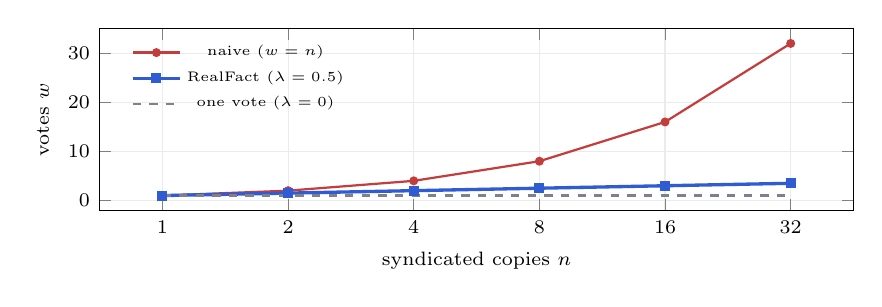
\begin{tikzpicture}
\begin{axis}[width=0.92\columnwidth,height=3.9cm,xlabel={syndicated copies $n$},ylabel={votes $w$},
  xmode=log,log basis x=2,xtick={1,2,4,8,16,32},xticklabels={1,2,4,8,16,32},
  legend pos=north west,legend style={font=\tiny,draw=none,fill=none},grid=major,grid style={black!8},
  tick label style={font=\scriptsize},label style={font=\scriptsize}]
\addplot[con,thick,mark=*,mark size=1.2pt] coordinates {(1,1)(2,2)(4,4)(8,8)(16,16)(32,32)}; \addlegendentry{naive ($w=n$)}
\addplot[novel,very thick,mark=square*,mark size=1.2pt] coordinates {(1,1)(2,1.5)(4,2)(8,2.5)(16,3)(32,3.5)}; \addlegendentry{RealFact ($\lambda=0.5$)}
\addplot[inkthree,dashed,thick] coordinates {(1,1)(32,1)}; \addlegendentry{one vote ($\lambda=0$)}
\end{axis}
\end{tikzpicture}
\caption{Cluster weight as a function of the number of syndicated copies.}
\label{fig:weights}
\end{figure}

\subsection{Verification history}
Every verdict is stored with its full result (evidence, weights, parameters, timings) in a separate SQLite database.
Past checks can be searched, reopened exactly as they were shown, re-run against today's corpus, or deleted.
Syndication stress-test runs are simulations and are not saved.

% =====================================================================================================
\section{Parallel Implementation}
\label{sec:par}

All three kernels use OpenMP~\cite{openmp} and live in one C++ file compiled twice: with OpenMP (\texttt{librealfact\_omp}) and without it
(\texttt{librealfact\_serial}). The serial build is the reference $T_1$, so OpenMP runtime overhead is not charged to
the baseline. Floating-point contraction is disabled (\texttt{-ffp-contract=off}) and every summation order is written
out explicitly, so both builds produce bit-identical results, which the test suite checks for every kernel.

\subsection{Kernel 1: exact top-$M$ scan}
The scan is a \texttt{parallel for} over corpus rows with \texttt{schedule(runtime)}, so the schedule kind and chunk
size are run-time parameters (Fig.~\ref{fig:k1}, Listing~\ref{lst:kernel}). Each thread keeps a private top-$M$
min-heap aligned and padded to a 64-byte cache line, which prevents false sharing on heap metadata. Ties are broken
by row index, making the order total and the output deterministic. The serial merge concatenates the $P$ local heaps
and applies \texttt{nth\_element} and a sort, $O(PM+M\log M)$, instead of the $O(PM\log M)$ heap merge first planned;
at 16 threads and $M=10{,}000$ this cut the 500K-row query from 11.46 to 9.48\,ms.

\begin{figure}[!t]
\centering
\resizebox{\columnwidth}{!}{%
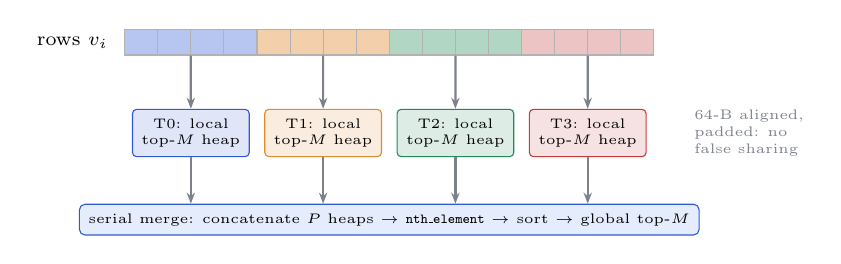
\begin{tikzpicture}[font=\scriptsize,
  row/.style={draw=black!30,minimum width=0.42cm,minimum height=0.32cm,inner sep=0},
  heap/.style={draw,rounded corners=1.5pt,minimum width=1.05cm,minimum height=0.5cm,align=center,font=\tiny},
  arr/.style={-{Stealth[length=1.4mm]},thick,inkthree}]
\foreach \i in {0,...,15} {
  \pgfmathtruncatemacro{\t}{int(\i/4)}
  \ifcase\t \def\c{tA!35}\or \def\c{tB!40}\or \def\c{sup!35}\or \def\c{con!30}\fi
  \node[row,fill=\c] (r\i) at (\i*0.42,0) {};
}
\node[anchor=east] at (-0.3,0) {rows $v_i$};
\foreach \t/\c/\n in {0/tA/T0,1/tB/T1,2/sup/T2,3/con/T3} {
  \node[heap,fill=\c!15,draw=\c] (h\t) at (0.63+\t*1.68,-1.15) {\n: local\\top-$M$ heap};
  \draw[arr] ($(r\the\numexpr\t*4\relax.south)!0.5!(r\the\numexpr\t*4+3\relax.south)$) -- (h\t.north);
}
\node[draw,rounded corners=2pt,fill=novelsoft,draw=novel,align=center,font=\tiny,minimum width=5.6cm] (m) at (3.15,-2.25)
  {serial merge: concatenate $P$ heaps $\to$ \texttt{nth\_element} $\to$ sort $\to$ global top-$M$};
\foreach \t in {0,...,3} \draw[arr] (h\t.south) -- (m.north -| h\t.south);
\node[font=\tiny,inkthree,align=left,anchor=west] at (6.9,-1.15) {64-B aligned,\\padded: no\\false sharing};
\end{tikzpicture}}
\caption{Kernel 1. Threads scan disjoint row ranges into private, cache-line-padded heaps; a serial merge independent
of $N$ produces the global top-$M$.}
\label{fig:k1}
\end{figure}

\begin{lstlisting}[language=C++,caption={Core of kernel 1 (\texttt{engine/realfact\_engine.cpp}).},label={lst:kernel},float=t]
struct alignas(64) LocalHeap { std::vector<Hit> h; /* + pad */ };
#pragma omp parallel num_threads(threads)
{
  LocalHeap& mine = heaps[omp_get_thread_num()];
  #pragma omp for schedule(runtime) nowait
  for (int64_t i = 0; i < N; ++i) {
    if (exclude && exclude[i]) continue;       // leakage mask
    mine.push(Hit{dot(q, emb + i*d, d), i}, M); // private top-M
  }
}  // serial merge: concatenate, nth_element, sort
\end{lstlisting}

\textbf{Dot product.} The first version accumulated each row into a single vector register, so each of its 96 vector
additions waited for the previous one (a loop-carried dependency) and one core ran at add \emph{latency}. The second
version keeps 16 independent partial sums, which compile to four independent 4-lane NEON registers, reduced by a
fixed tree. The order is explicit, so no \texttt{-ffast-math} is needed and the builds stay bit-exact. A register-blocked
\texttt{dot4} scores four vectors per row load and is bit-identical to \texttt{dot}; it powers the multi-query batch
kernel and kernels 2 and 3.

\subsection{Kernel 2: all-pairs syndication detection}
To measure redundancy across the whole corpus, kernel 2 compares every pair $i<j$ once, links pairs with cosine
above $\tau$, and forms connected components with union-find~\cite{tarjan}. Rows are processed in blocks of four
against each partner row with \texttt{dot4}, so every partner row loaded from memory is used four times; the kernel
is compute-bound, unlike the scan. Edges go to per-thread buffers without locks, then are concatenated and sorted, so
the output is deterministic. The merge and union-find are serial and timed separately as the Amdahl~\cite{amdahl} term.

The iteration space is a triangle: row block $b$ has about $N-4b$ partners. Fig.~\ref{fig:tri} shows why the schedule
matters. With \texttt{static} and the default chunk, each thread receives one contiguous range of rows, and the first
range carries most of the work. Interleaving rows (\texttt{static,1}) or handing them out on demand
(\texttt{dynamic}, \texttt{guided}) balances the triangle.

\begin{figure}[!t]
\centering
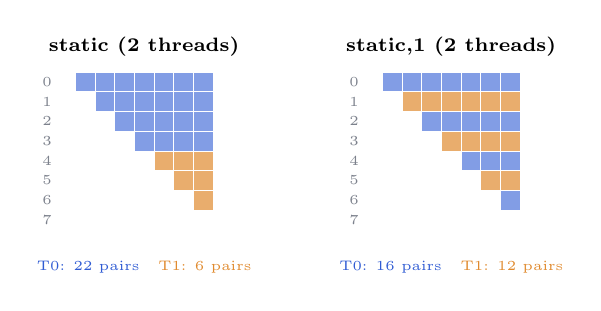
\begin{tikzpicture}[font=\tiny,cell/.style={minimum size=0.25cm,inner sep=0,draw=white,line width=0.3pt}]
\def\n{8}
\begin{scope}
\node[font=\scriptsize\bfseries] at (1.0,0.45) {static (2 threads)};
\foreach \i in {0,...,7} {
  \pgfmathtruncatemacro{\own}{\i<4 ? 0 : 1}
  \ifnum\own=0 \def\c{tA!60}\else\def\c{tB!70}\fi
  \foreach \j in {0,...,7} { \ifnum\j>\i \node[cell,fill=\c] at (\j*0.25,-\i*0.25) {}; \fi }
  \node[anchor=east,inkthree] at (-0.05,-\i*0.25) {\i};
}
\node[align=center] at (1.0,-2.35) {\textcolor{tA}{T0: 22 pairs}\quad\textcolor{tB}{T1: 6 pairs}};
\end{scope}
\begin{scope}[xshift=3.9cm]
\node[font=\scriptsize\bfseries] at (1.0,0.45) {static,1 (2 threads)};
\foreach \i in {0,...,7} {
  \pgfmathtruncatemacro{\own}{mod(\i,2)}
  \ifnum\own=0 \def\c{tA!60}\else\def\c{tB!70}\fi
  \foreach \j in {0,...,7} { \ifnum\j>\i \node[cell,fill=\c] at (\j*0.25,-\i*0.25) {}; \fi }
  \node[anchor=east,inkthree] at (-0.05,-\i*0.25) {\i};
}
\node[align=center] at (1.0,-2.35) {\textcolor{tA}{T0: 16 pairs}\quad\textcolor{tB}{T1: 12 pairs}};
\end{scope}
\end{tikzpicture}
\caption{Kernel 2's triangular iteration space for $N=8$ rows (cell $(i,j)$ = one pair). Contiguous static ranges
give thread 0 3.7$\times$ the work of thread 1; cyclic assignment narrows the gap; dynamic scheduling closes it.}
\label{fig:tri}
\end{figure}

\subsection{Kernel 3: block-speculative leader clustering}
Algorithm~\ref{alg:cluster} has a loop-carried dependency: whether candidate $j$ founds a cluster depends on every
leader founded before it, so its loop cannot simply be parallelised. Kernel 3 uses block speculation
(Fig.~\ref{fig:spec}). For a block of $B$ candidates, the similarity of each candidate to the leaders that exist at
block start is computed in parallel. A short sequential walk then compares each candidate only with leaders founded
inside the block and makes the decision. Leaders are compared in founding order with a strict ``$>$'' throughout, so
the arg-max and the output are exactly those of the sequential algorithm. Once $K$ leaders exist, assigning the
remaining pool is a regular parallel loop. Parallel regions are skipped below 4,096 dot products, where fork/join
would cost more than the work.

\begin{figure}[!t]
\centering
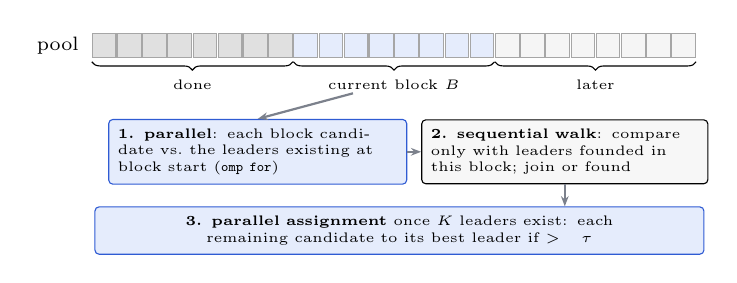
\begin{tikzpicture}[font=\tiny,
  c/.style={draw=black!35,minimum width=0.3cm,minimum height=0.3cm,inner sep=0},
  arr/.style={-{Stealth[length=1.3mm]},thick,inkthree}]
\foreach \i in {0,...,23} {
  \pgfmathtruncatemacro{\blk}{int(\i/8)}
  \ifcase\blk \def\f{black!12}\or \def\f{novelsoft}\or \def\f{black!4}\fi
  \node[c,fill=\f] (k\i) at (\i*0.32,0) {};
}
\node[anchor=east,font=\scriptsize] at (-0.2,0) {pool};
\draw[decorate,decoration={brace,amplitude=3pt,mirror}] ($(k0.south west)+(0,-0.05)$) -- ($(k7.south east)+(0,-0.05)$) node[midway,below=3pt] {done};
\draw[decorate,decoration={brace,amplitude=3pt,mirror}] ($(k8.south west)+(0,-0.05)$) -- ($(k15.south east)+(0,-0.05)$) node[midway,below=3pt] {current block $B$};
\draw[decorate,decoration={brace,amplitude=3pt,mirror}] ($(k16.south west)+(0,-0.05)$) -- ($(k23.south east)+(0,-0.05)$) node[midway,below=3pt] {later};
\node[draw=novel,fill=novelsoft,rounded corners=1.5pt,align=left,text width=3.55cm] (p1) at (1.95,-1.35)
  {\textbf{1. parallel}: each block candidate vs.\ the leaders existing at block start (\texttt{omp for})};
\node[draw,fill=black!3,rounded corners=1.5pt,align=left,text width=3.4cm] (p2) at (5.85,-1.35)
  {\textbf{2. sequential walk}: compare only with leaders founded in this block; join or found};
\draw[arr] (p1) -- (p2);
\draw[arr] ($(k8.south)+(0.6,-0.45)$) -- (p1.north);
\node[draw=novel,fill=novelsoft,rounded corners=1.5pt,align=center,text width=7.5cm] (p3) at (3.75,-2.35)
  {\textbf{3. parallel assignment} once $K$ leaders exist: each remaining candidate to its best leader if $>\tau$};
\draw[arr] (p2.south) -- (p2.south |- p3.north);
\end{tikzpicture}
\caption{Kernel 3. Block speculation turns the sequential leader loop into parallel similarity work plus a short
sequential decision pass, with output identical to Algorithm~\ref{alg:cluster}.}
\label{fig:spec}
\end{figure}

\subsection{Engineering issues}
Apple clang ships no OpenMP runtime, so we link a prebuilt LLVM libomp 19.1.5. PyTorch bundles its own libomp, and if
it initialises first our runtime crashes on its first parallel region, so the engine libraries are loaded before any
PyTorch import. Benchmarks and ingestion share a lock: an early sweep that overlapped with embedding showed more than
100\% CPU utilisation on one thread. macOS exposes no thread-affinity API, so \texttt{OMP\_PROC\_BIND} has no effect;
we disclose this rather than claim pinned results.

% =====================================================================================================
\section{Experimental Setup}
\label{sec:setup}

\begin{table}[!t]
\caption{Platform disclosure}
\label{tab:platform}
\centering\footnotesize
\setlength{\tabcolsep}{3pt}
\begin{tabularx}{\columnwidth}{lY}
\toprule
CPU & Apple M3 Pro, 11 cores (5 performance + 6 efficiency), no SMT\\
Caches & L1d 64\,KB; L2 16\,MB (P cluster), 4\,MB (E cluster)\\
Memory & 18\,GB unified\\
Compiler & Apple clang 21, \texttt{-O3 -std=c++17 -ffp-contract=off}\\
OpenMP & LLVM libomp 19.1.5; max 11 threads; no pinning on macOS\\
Models & BGE-small-en-v1.5~\cite{bge} (384-d); NLI: nli-deberta-v3-xsmall (news), DeBERTa-v3-base-mnli-fever-anli~\cite{laurer} (FEVER)\\
\bottomrule
\end{tabularx}
\end{table}

\textbf{Protocol.} Kernel 1 is timed under static, dynamic and guided scheduling at 1, 2, 4, 8 and 16 threads on the
live corpus and on synthetic corpora of 10K--500K random unit vectors (retrieval cost depends only on $N\times d$),
with $M=10{,}000$. Each configuration runs 2 discarded warm-ups and 11 timed queries; we report medians, IQR and p95,
and compare schedules with an exact two-sided Wilcoxon signed-rank test on paired per-query latencies. Kernel 2 is
timed under static, static,1, dynamic and guided at 1, 2, 4, 8 and 11 threads on the live corpus and a 10K synthetic
corpus, median of 5 runs after a warm-up. Kernel 3 is timed on a 8,983-candidate pool shaped like real syndication
(2,000 stories with 1--8 near-copies each). For every configuration of every kernel, output is compared with the
serial build.

\textbf{Roofline expectation~\cite{roofline}.} One scan query performs 2 flops per 4-byte value read (0.5 flop/byte), so kernel 1 is
memory-bound; its 500K-row working set (768\,MB) exceeds every cache. Kernel 2 reuses each row against thousands of
partners and should be compute-bound.

% =====================================================================================================
\section{Results}
\label{sec:results}

\subsection{Kernel 1: strong scaling of the original kernel}
Fig.~\ref{fig:speedup} shows speedup and efficiency of the first version (v1) at $N=500{,}000$. Guided reaches
$4.61\times$ at 16 threads (9.48\,ms against 43.68\,ms serial), static $3.78\times$, and dynamic with the default
chunk of 1 only $1.16\times$, because it pays an atomic increment per row. Efficiency is 79\% at 4 threads and falls
beyond, where the kernel approaches the memory-bandwidth ceiling (81\,GB/s at 16 threads against 17.6\,GB/s on one
thread). Across 5 corpus sizes $\times$ 15 configurations $\times$ 11 queries the returned IDs were bit-identical to the
serial build in every case.

\begin{figure}[!t]
\centering
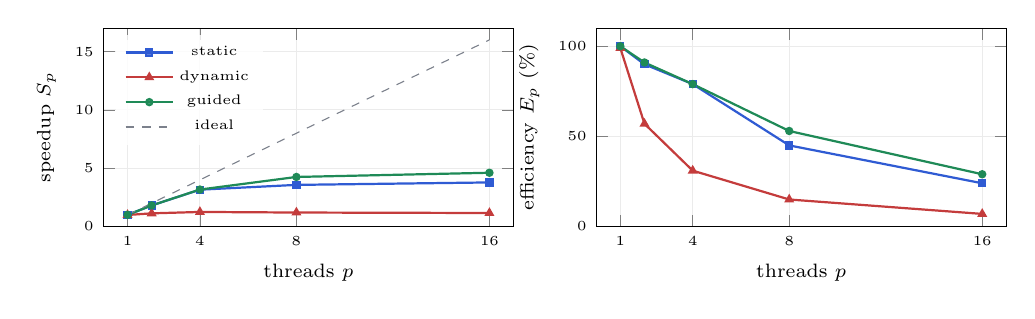
\begin{tikzpicture}
\begin{groupplot}[group style={group size=2 by 1,horizontal sep=1.05cm},
  width=0.56\columnwidth,height=4.1cm,xlabel={threads $p$},xtick={1,4,8,16},xmin=0,xmax=17,
  grid=major,grid style={black!8},tick label style={font=\tiny},label style={font=\scriptsize},
  legend style={font=\tiny,draw=none,fill=white,fill opacity=0.8,text opacity=1}]
\nextgroupplot[ylabel={speedup $S_p$},ymin=0,ymax=17,legend pos=north west]
\addplot[novel,thick,mark=square*,mark size=1.1pt] coordinates {(1,1.00)(2,1.81)(4,3.16)(8,3.57)(16,3.78)}; \addlegendentry{static}
\addplot[con,thick,mark=triangle*,mark size=1.3pt] coordinates {(1,0.99)(2,1.13)(4,1.25)(8,1.20)(16,1.16)}; \addlegendentry{dynamic}
\addplot[sup,thick,mark=*,mark size=1.1pt] coordinates {(1,1.00)(2,1.81)(4,3.17)(8,4.25)(16,4.61)}; \addlegendentry{guided}
\addplot[inkthree,dashed] coordinates {(1,1)(16,16)}; \addlegendentry{ideal}
\nextgroupplot[ylabel={efficiency $E_p$ (\%)},ymin=0,ymax=110]
\addplot[novel,thick,mark=square*,mark size=1.1pt] coordinates {(1,100)(2,90)(4,79)(8,45)(16,24)};
\addplot[con,thick,mark=triangle*,mark size=1.3pt] coordinates {(1,99)(2,57)(4,31)(8,15)(16,7)};
\addplot[sup,thick,mark=*,mark size=1.1pt] coordinates {(1,100)(2,91)(4,79)(8,53)(16,29)};
\end{groupplot}
\end{tikzpicture}
\caption{Kernel 1 (v1) at $N=500{,}000$, $M=10{,}000$: speedup and efficiency against the non-OpenMP build ($T_1=43.68$\,ms).}
\label{fig:speedup}
\end{figure}

Guided beats static at 8 and 16 threads (exact Wilcoxon $p=9.8\times10^{-4}$, $r=0.88$ at 500K, the smallest $p$
attainable with $n=11$), contrary to the textbook expectation for uniform work. The cause is the heterogeneous CPU:
static gives every core an equal share, so threads on efficiency cores finish last. At 1,725 rows the best speedup
is $1.7\times$, since thread start-up costs about as much as the 0.22\,ms scan.

\subsection{Kernel 1: course-driven optimisations}
\textbf{ILP rewrite.} The 16-accumulator dot product made the serial scan $2.60\times$ faster (43.68 to 16.82\,ms;
17.6 to 45.7\,GB/s on one core) and the best parallel time $1.18\times$ faster (8.04\,ms, 96\,GB/s, static at 8
threads). Speedup over the new $T_1$ fell to $2.09\times$ because the faster core reaches the shared bandwidth ceiling
with only 4 threads (Table~\ref{tab:v1v2}): optimising the serial code raised the baseline, which is why speedup must be
read next to its baseline.

\begin{table}[!t]
\caption{Kernel 1, v1 to v2, at $N=500{,}000$ (medians of 11 runs)}
\label{tab:v1v2}
\centering\footnotesize
\resizebox{\columnwidth}{!}{%
\begin{tabular}{lrrr}
\toprule
& \textbf{v1} & \textbf{v2} & \textbf{change}\\
\midrule
Serial $T_1$ & 43.68\,ms & 16.82\,ms & $2.60\times$ faster\\
One-core bandwidth & 17.6\,GB/s & 45.7\,GB/s & \\
Best parallel time & 9.48\,ms & 8.04\,ms & $1.18\times$ faster\\
Bandwidth at best & 81\,GB/s & 96\,GB/s & \\
Speedup over own $T_1$ & $4.61\times$ & $2.09\times$ & lower\\
Threads to 90\% of best & 16 & 4 & \\
\bottomrule
\end{tabular}}
\end{table}

\textbf{Karp--Flatt.} The serial fraction $e=(1/S_p-1/p)/(1-1/p)$~\cite{karpflatt} for v2 static rises from 0.27 at
$p=2$ to 0.49 at $p=16$. A rising $e$ indicates overhead that grows with $p$, here contention for memory bandwidth,
not a fixed serial section (the only serial code, the heap merge, takes about 0.1\,ms).

\textbf{Load balance.} Per-thread busy time measured inside the worksharing loop with padded counters
(Table~\ref{tab:lb}) shows static leaving threads idle 11\% of the loop at 11 threads, while guided and chunked
dynamic let fast cores take up to $1.9\times$ more rows and finish within 1--2\% of one another. Dynamic with chunk 1
is balanced but $4.9\times$ slower. A chunk sweep showed dynamic needs at least about 256 rows per chunk; guided is
best at its default.

\begin{table}[!t]
\caption{Kernel 1 load balance at 11 threads, $N=500{,}000$}
\label{tab:lb}
\centering\footnotesize
\setlength{\tabcolsep}{3.5pt}
\resizebox{\columnwidth}{!}{%
\begin{tabular}{lrrrr}
\toprule
\textbf{Schedule} & \textbf{ms} & \textbf{max/mean busy} & \textbf{Idle} & \textbf{Rows per thread}\\
\midrule
static & 9.14 & 1.12 & 11\% & 45,454--45,455\\
dynamic, chunk 1 & 39.99 & 1.01 & 1\% & 40,489--51,814\\
dynamic, chunk 4096 & 8.74 & 1.02 & 2\% & 20,480--69,632\\
guided & \textbf{8.15} & 1.01 & 1\% & 31,554--58,761\\
\bottomrule
\end{tabular}}
\end{table}

\textbf{Weak scaling.} With 31,250 rows per thread, weak efficiency~\cite{gustafson} (guided) is 98\% at 2 threads,
87\% at 4, 51\% at 8 and 26\% at 16: the same bandwidth ceiling limits weak and strong scaling, so for a
bandwidth-bound kernel Gustafson's law offers no escape.

\textbf{Roofline and multi-query blocking.} Scoring $Q$ queries per row load raises arithmetic intensity to $0.5Q$
flop/byte. With $M=100$, throughput rises from 139 to 688 queries/s ($4.9\times$) and the kernel leaves the bandwidth
roof at $Q\approx4$ (Fig.~\ref{fig:roofline}). With $M=10{,}000$ heap maintenance dominates and the gain is small.

\begin{figure}[!t]
\centering
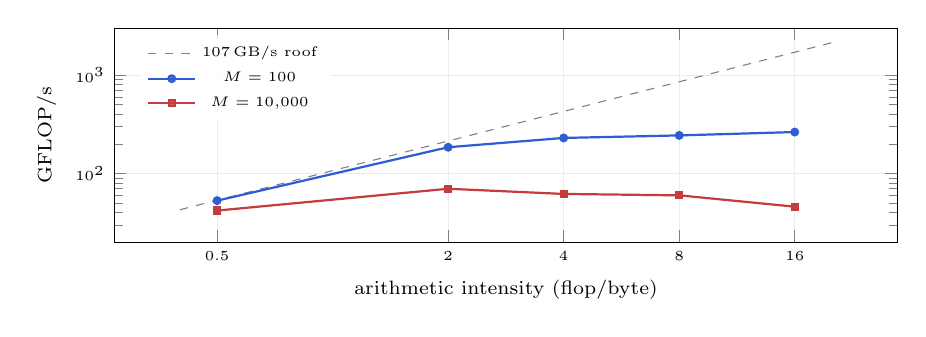
\begin{tikzpicture}
\begin{axis}[width=0.95\columnwidth,height=4.3cm,xmode=log,ymode=log,log basis x=2,
  xlabel={arithmetic intensity (flop/byte)},ylabel={GFLOP/s},xtick={0.5,2,4,8,16},xticklabels={0.5,2,4,8,16},
  legend pos=north west,ymin=20,ymax=3000,grid=major,grid style={black!8},tick label style={font=\tiny},
  label style={font=\scriptsize},legend style={font=\tiny,draw=none,fill=white,fill opacity=0.8,text opacity=1}]
\addplot[inkthree,dashed,domain=0.4:20,samples=2] {107*x}; \addlegendentry{107\,GB/s roof}
\addplot[novel,thick,mark=*,mark size=1.2pt] coordinates {(0.5,53)(2,185)(4,230)(8,244)(16,264)}; \addlegendentry{$M=100$}
\addplot[con,thick,mark=square*,mark size=1.1pt] coordinates {(0.5,42)(2,70)(4,62)(8,60)(16,46)}; \addlegendentry{$M=10{,}000$}
\end{axis}
\end{tikzpicture}
\caption{Roofline of kernel 1 with multi-query blocking ($Q=1..32$) at 16 threads, $N=500{,}000$.}
\label{fig:roofline}
\end{figure}

\textbf{Adaptive threads.} Verification now uses $p=\min(\text{cores},8,\lceil N/400\rceil)$ threads with the guided
schedule: enough rows per thread to amortise fork/join, and no more threads than the memory system can feed.

\subsection{Kernel 2: all-pairs syndication detection}
Fig.~\ref{fig:k2} and Table~\ref{tab:k2} report kernel 2. The serial build runs at about 48\,GFLOP/s. On the live
corpus (3,635 articles, 6.6M pairs) dynamic reaches $6.92\times$ at 11 threads (15.4\,ms against 106.5\,ms), guided
$6.69\times$, static,1 $5.56\times$, and static only $4.98\times$, because its busiest thread does $1.90\times$ the
average work, exactly the triangular imbalance of Fig.~\ref{fig:tri}. The 10K synthetic corpus (50M pairs) shows the
same ordering. The serial merge and union-find take under 0.15\% of the parallel time, so Amdahl's serial fraction is
not the limit. The limit is the hardware: 5 threads on performance cores give $4.6\times$, and each efficiency core
adds roughly 40\% of a performance core, so 11 threads are worth about 7 performance cores. Every one of the 40
configurations produced edges and groups identical to the serial build.

\begin{figure}[!t]
\centering
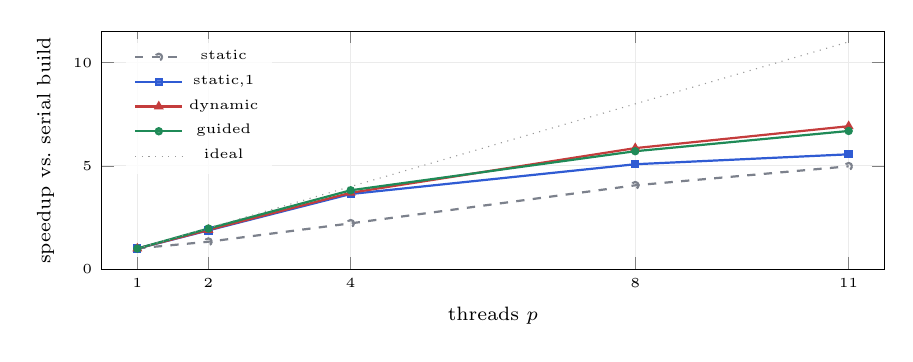
\begin{tikzpicture}
\begin{axis}[width=0.95\columnwidth,height=4.6cm,xlabel={threads $p$},ylabel={speedup vs.\ serial build},
  xtick={1,2,4,8,11},xmin=0.5,xmax=11.5,ymin=0,ymax=11.5,grid=major,grid style={black!8},
  tick label style={font=\tiny},label style={font=\scriptsize},legend pos=north west,
  legend style={font=\tiny,draw=none,fill=white,fill opacity=0.8,text opacity=1}]
\addplot[inkthree,thick,dashed,mark=o,mark size=1.2pt] coordinates {(1,1.01)(2,1.33)(4,2.22)(8,4.06)(11,4.98)}; \addlegendentry{static}
\addplot[novel,thick,mark=square*,mark size=1.1pt] coordinates {(1,1.00)(2,1.88)(4,3.64)(8,5.08)(11,5.56)}; \addlegendentry{static,1}
\addplot[con,thick,mark=triangle*,mark size=1.3pt] coordinates {(1,1.00)(2,1.90)(4,3.70)(8,5.86)(11,6.92)}; \addlegendentry{dynamic}
\addplot[sup,thick,mark=*,mark size=1.1pt] coordinates {(1,1.00)(2,1.97)(4,3.82)(8,5.71)(11,6.69)}; \addlegendentry{guided}
\addplot[black!40,dotted] coordinates {(1,1)(11,11)}; \addlegendentry{ideal}
\end{axis}
\end{tikzpicture}
\caption{Kernel 2 on the live corpus (3,635 articles, 6.6M pairs).}
\label{fig:k2}
\end{figure}

\begin{table}[!t]
\caption{Kernel 2 at 11 threads: speedup and busiest-thread load (max/mean busy time)}
\label{tab:k2}
\centering\footnotesize
\setlength{\tabcolsep}{3.5pt}
\begin{tabular}{lrrrrrr}
\toprule
& \multicolumn{3}{c}{\textbf{Live, 6.6M pairs}} & \multicolumn{3}{c}{\textbf{Synthetic, 50M pairs}}\\
\cmidrule(lr){2-4}\cmidrule(lr){5-7}
\textbf{Schedule} & \textbf{ms} & $S_p$ & \textbf{max/mean} & \textbf{ms} & $S_p$ & \textbf{max/mean}\\
\midrule
serial & 106.5 & 1.00 & --- & 809.3 & 1.00 & ---\\
static & 21.36 & 4.98 & 1.90 & 168.70 & 4.80 & 1.76\\
static,1 & 19.16 & 5.56 & 1.37 & 129.88 & 6.23 & 1.11\\
dynamic & \textbf{15.40} & \textbf{6.92} & 1.00 & \textbf{126.01} & \textbf{6.42} & 1.00\\
guided & 15.91 & 6.69 & 1.12 & 127.18 & 6.36 & 1.00\\
\bottomrule
\end{tabular}
\end{table}

On the live corpus at $\tau=0.9$, 13.1\% of articles have a near-copy, forming 187 groups; the largest is one story
carried as 23 articles across 10 outlets (Fig.~\ref{fig:ui-corpus}a). Under naive counting that story would count as 23
confirmations; RealFact gives it $1+0.5\log_2 23=3.26$ votes.

\subsection{Kernel 3: parallel leader clustering}
Table~\ref{tab:k3} compares kernel 3 with the serial build and with the NumPy reference implementation of
Algorithm~\ref{alg:cluster}, whose assignment step is a matrix product executed by Apple's Accelerate BLAS. All 15
configurations returned output identical to the reference. At the default $K=10$, 11 threads are $5.8\times$ faster
than the serial build and $3.2\times$ faster than NumPy. At $K=1000$ the kernel is $2.5\times$ faster than NumPy. At
$K=100$ NumPy is faster ($0.75\times$): its matrix product runs on the M3's dedicated matrix unit, a hardware
accelerator rather than more CPU parallelism. On the live corpus the pool above the relevance floor is usually a few
dozen articles, so the stage takes microseconds and stays serial by design.

\begin{table}[!t]
\caption{Kernel 3 on a pool of 8,983 syndicated candidates (median ms)}
\label{tab:k3}
\centering\footnotesize
\setlength{\tabcolsep}{3.2pt}
\resizebox{\columnwidth}{!}{%
\begin{tabular}{rrrrrrrr}
\toprule
$K$ & \textbf{NumPy} & \textbf{serial} & \textbf{2T} & \textbf{4T} & \textbf{11T} & \textbf{vs serial} & \textbf{vs NumPy}\\
\midrule
10 & 0.96 & 1.72 & 0.89 & 0.47 & 0.30 & $5.8\times$ & \textcolor{sup}{$3.2\times$}\\
100 & 2.04 & 17.84 & 9.11 & 4.70 & 2.73 & $6.5\times$ & \textcolor{con}{$0.75\times$}\\
1000 & 74.29 & 191.32 & 99.22 & 52.71 & 29.82 & $6.4\times$ & \textcolor{sup}{$2.5\times$}\\
\bottomrule
\end{tabular}}
\end{table}

\subsection{Correctness}
Table~\ref{tab:tests} lists the 14-check suite, runnable from the command line or the benchmark tab. All checks pass
for every kernel version reported here.

\begin{table}[!t]
\caption{Correctness suite (\texttt{tests/test\_correctness.py}); all 14 pass}
\label{tab:tests}
\centering\footnotesize
\setlength{\tabcolsep}{3pt}
\begin{tabularx}{\columnwidth}{P{2.35cm}Y}
\toprule
\textbf{Check} & \textbf{What it verifies}\\
\midrule
Scan vs NumPy & 45 schedule $\times$ thread $\times$ chunk configurations return the exact top-$M$.\\
Bit-exactness & 36 parallel runs identical to the serial build at $M=10{,}000$.\\
Ties, edge cases & 40-way tie in index order; $M>N$, $N\in\{0,1\}$, odd $d$.\\
Leakage mask & Masked rows are never returned.\\
Batch, accounting & Batched = single query; per-thread rows sum to $N$.\\
Aggregation & $S$, $D$ and verdicts on hand-computed cases.\\
Kernel 3 & 162 configurations identical to the NumPy reference.\\
Kernel 2 & Edges equal a float64 Gram matrix, groups equal BFS, pairs covered exactly once.\\
Statistics, data & Exact Wilcoxon vs enumeration; ingestion keys; label maps.\\
\bottomrule
\end{tabularx}
\end{table}

\subsection{Independence filter: controlled syndication test}
The interface can republish one real article as $n$ near-identical copies under labelled simulated outlets, for one
query; the copies are appended to the matrix kernel 1 scans. For the claim ``Kuwait-flagged tanker with 21 Indian
seafarers hit near Strait of Hormuz, crew safe'', four independent clusters were retrieved (one SUPPORT, two NEUTRAL,
one CONTRADICT) and the verdict was Conflicting Evidence. After republishing the contradicting article $\times10$
(Table~\ref{tab:case}), naive counting and raw top-$K$ flip to Contradicted, while RealFact counts the 11-copy cluster
as 2.73 votes and correctly stays Conflicting Evidence. On unmodified data all rules agree
(Fig.~\ref{fig:ui-cards}b), the expected control: cross-outlet reports score 0.75--0.88, below $\tau$, and are
independent reports, not copies.

\begin{table}[!t]
\caption{Same evidence after syndicating the contradicting article $\times10$}
\label{tab:case}
\centering\footnotesize
\setlength{\tabcolsep}{3pt}
\begin{tabular}{lcrrr}
\toprule
\textbf{Aggregation rule} & \textbf{Verdict} & $S$ & $D$ & $\sum w$\\
\midrule
\rowcolor{novelsoft}RealFact ($\lambda=0.5$) & \textcolor{conf}{\textbf{Conflicting}} & $-0.22$ & 0.31 & 6.2\\
One vote per cluster & \textcolor{conf}{Conflicting} & $0.04$ & 0.55 & 4.0\\
Naive counting & \textcolor{con}{Contradicted} & $-0.62$ & 0.10 & 15.0\\
Raw top-$K$ & \textcolor{con}{Contradicted} & $-0.56$ & 0.14 & 10.0\\
\bottomrule
\end{tabular}
\end{table}

\subsection{Verification quality}
\label{sec:fever}
\textbf{LIAR.} On the 1,267 labelled test statements against the live corpus, 99.1\% came back Unverified and accuracy
equalled the majority-class baseline (37.6\%). LIAR's claims date from 2007--2016 and the corpus covers a few days of
current news, so this run measures corpus coverage, not reasoning: the system correctly declines to guess.

\textbf{FEVER demo subset.} To test reasoning with a matched evidence pool we built a corpus of 25,324 pages from the
FEVER 2017 dump: the gold pages of 179 dev claims (60 SUPPORTS, 59 REFUTES, 60 NOT ENOUGH INFO), 2,723 pages cited by
other dev claims as hard distractors, and 22,476 random pages. SUPPORTS and REFUTES claims were selected with evidence
in a page's first four sentences, because the index embeds page leads. The NLI model~\cite{laurer} is trained on
FEVER's train split, so testing on dev claims is fair.

All tuning used a \emph{separate} split of 180 other dev claims that share no claim or gold page with the 179 test
claims; the test claims were scored once afterwards. Three changes were chosen on that split: sentence-level NLI
(each sentence of a page is checked and the most decisive one is used, as FEVER systems select sentences), a relative
cutoff keeping clusters within 0.04 cosine of the best match (still up to $K=10$), and $\theta=0.8$ with a relevance
floor of 0.64. A larger DeBERTa-v3-large NLI model was no better on the tuning split and 2--3$\times$ slower.
Table~\ref{tab:fever} reports the result: 81.0\% accuracy (macro F1 0.807) against 74.3\% before tuning, with the
gold page ranked first for 92.4\% of verifiable claims. The tuning split scores 83.9\%, close to the test result, as
expected when settings are not fitted to the test claims. Remaining errors are mostly NOT ENOUGH INFO claims labelled
Contradicted (15 of 60), whose pages exist and partly conflict with the claim. Being curated for lead-only evidence,
the subset is not comparable to published full-FEVER scores.

\begin{table}[!t]
\caption{FEVER demo subset: 179 test claims, 25,324 pages ($^\dagger$settings chosen on the held-out tuning split)}
\label{tab:fever}
\centering\footnotesize
\setlength{\tabcolsep}{3pt}
\begin{tabular}{lrrrr}
\toprule
\textbf{Configuration} & \textbf{Acc.} & \textbf{F1} & \textbf{ms} & \textbf{R@1}\\
\midrule
xsmall NLI, paragraph, default & 58.7\% & 0.585 & 65 & 89.1\%\\
FEVER NLI, paragraph, default & 74.3\% & 0.741 & 95 & 89.1\%\\
\rowcolor{novelsoft}FEVER NLI, sentence, tuned$^\dagger$ & \textbf{81.0\%} & \textbf{0.807} & 114 & 92.4\%\\
\bottomrule
\end{tabular}
\end{table}

\textbf{Latency.} A typical live claim takes about 100--125\,ms end to end: claim embedding 8--20\,ms, kernel 1
0.4\,ms, kernel 3 under 0.01\,ms, NLI about 90--110\,ms, aggregation under 0.1\,ms; web search, when enabled, adds
1--3\,s. NLI dominates at the current corpus size; kernel 1 becomes significant at hundreds of thousands of articles,
where it costs 8--44\,ms per query.

% =====================================================================================================
\section{User Interface}
The single-page interface has six tabs: \emph{Verify a claim}, \emph{Existing vs RealFact}, \emph{Parallel benchmark},
\emph{Live corpus}, \emph{Evaluation} and \emph{History}. Figs.~\ref{fig:ui-verdict}, \ref{fig:ui-cards} and \ref{fig:ui-corpus}
are screenshots of the running system.

\begin{figure*}[!t]
\centering
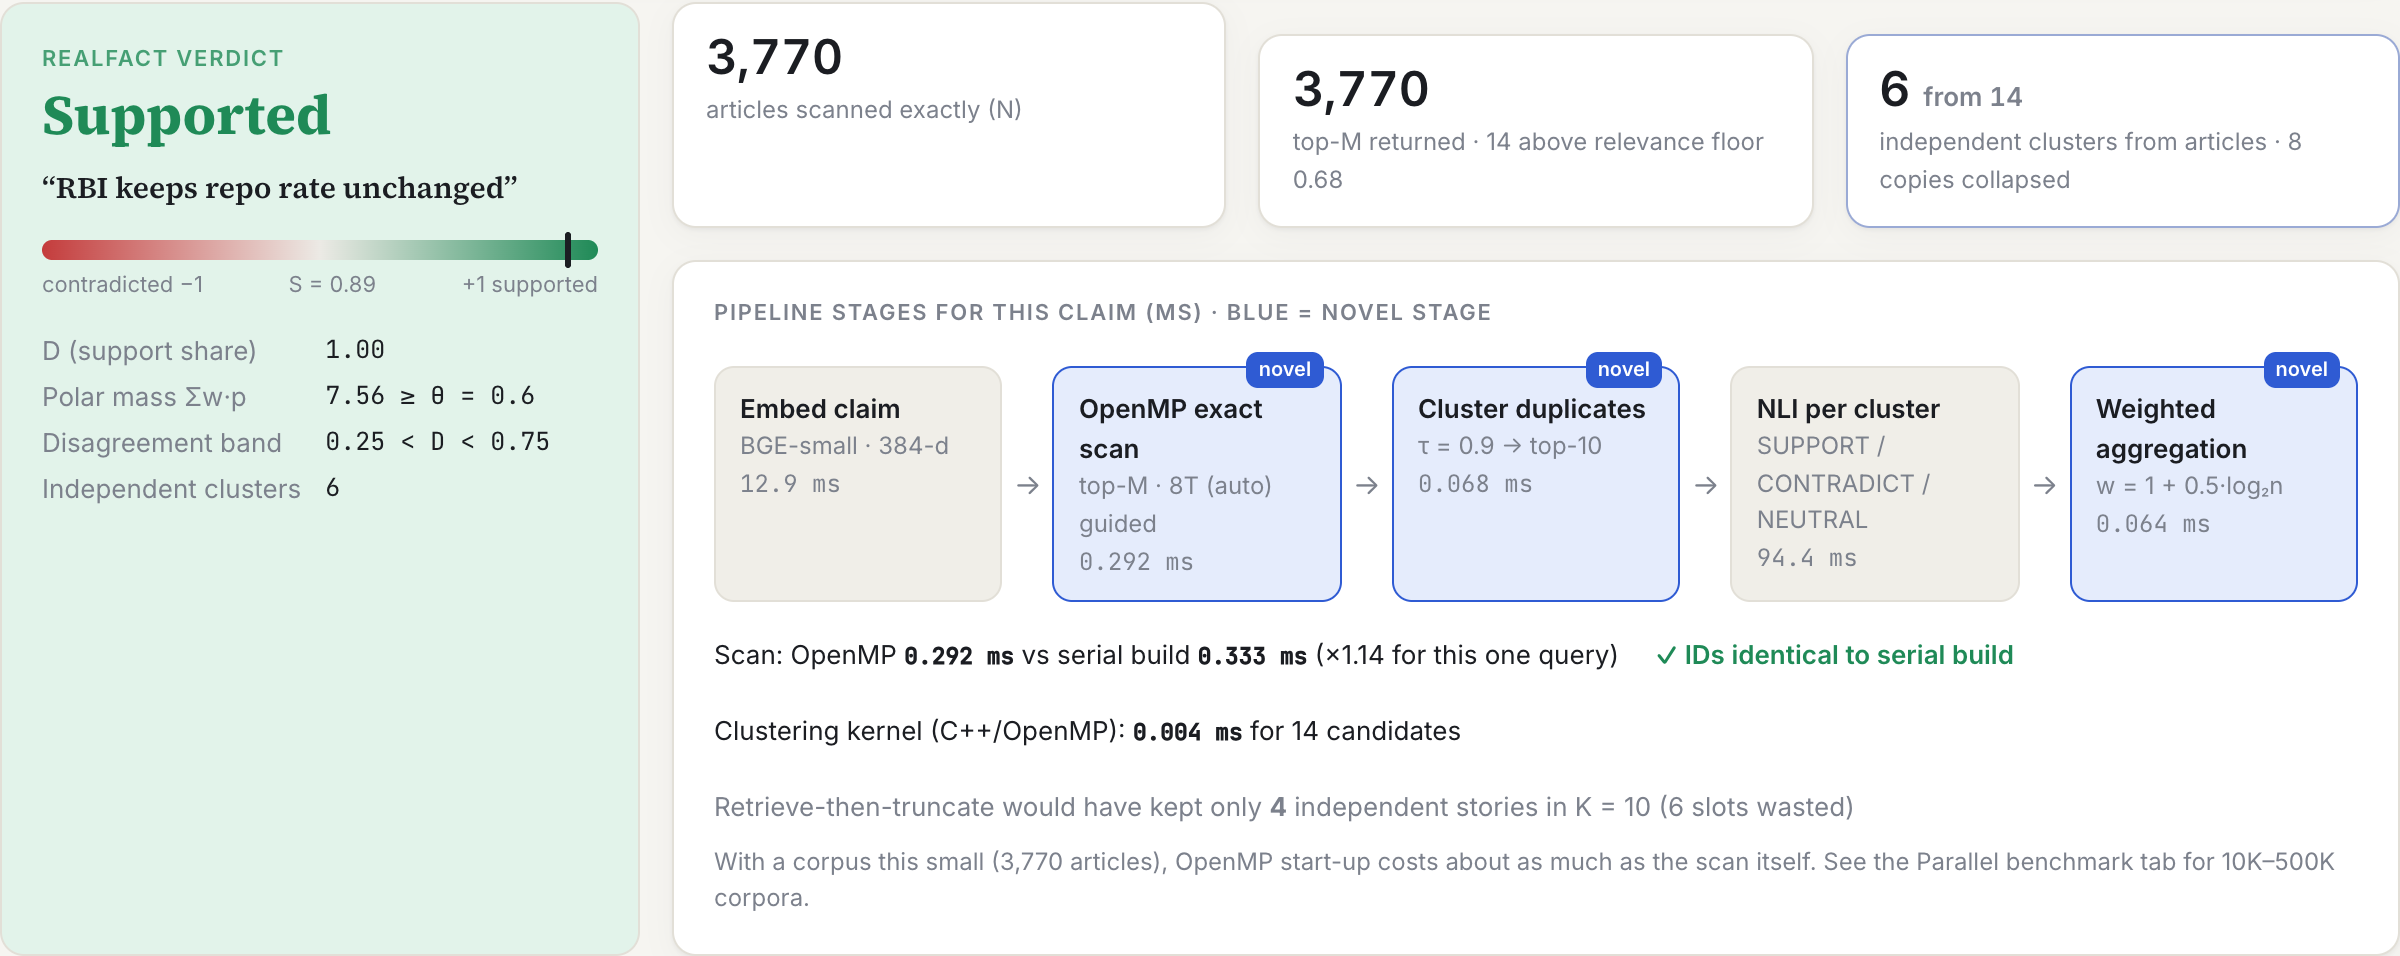
\includegraphics[width=0.92\textwidth]{ui_verdict.png}
\caption{Verify tab: verdict panel with the $S$ meter and $D$, polar mass and cluster count; corpus statistics; and the
timed pipeline stages (blue = novel stage), with the per-query OpenMP vs.\ serial comparison and the retrieve-then-truncate
counterfactual.}
\label{fig:ui-verdict}
\end{figure*}

\begin{figure*}[!t]
\centering
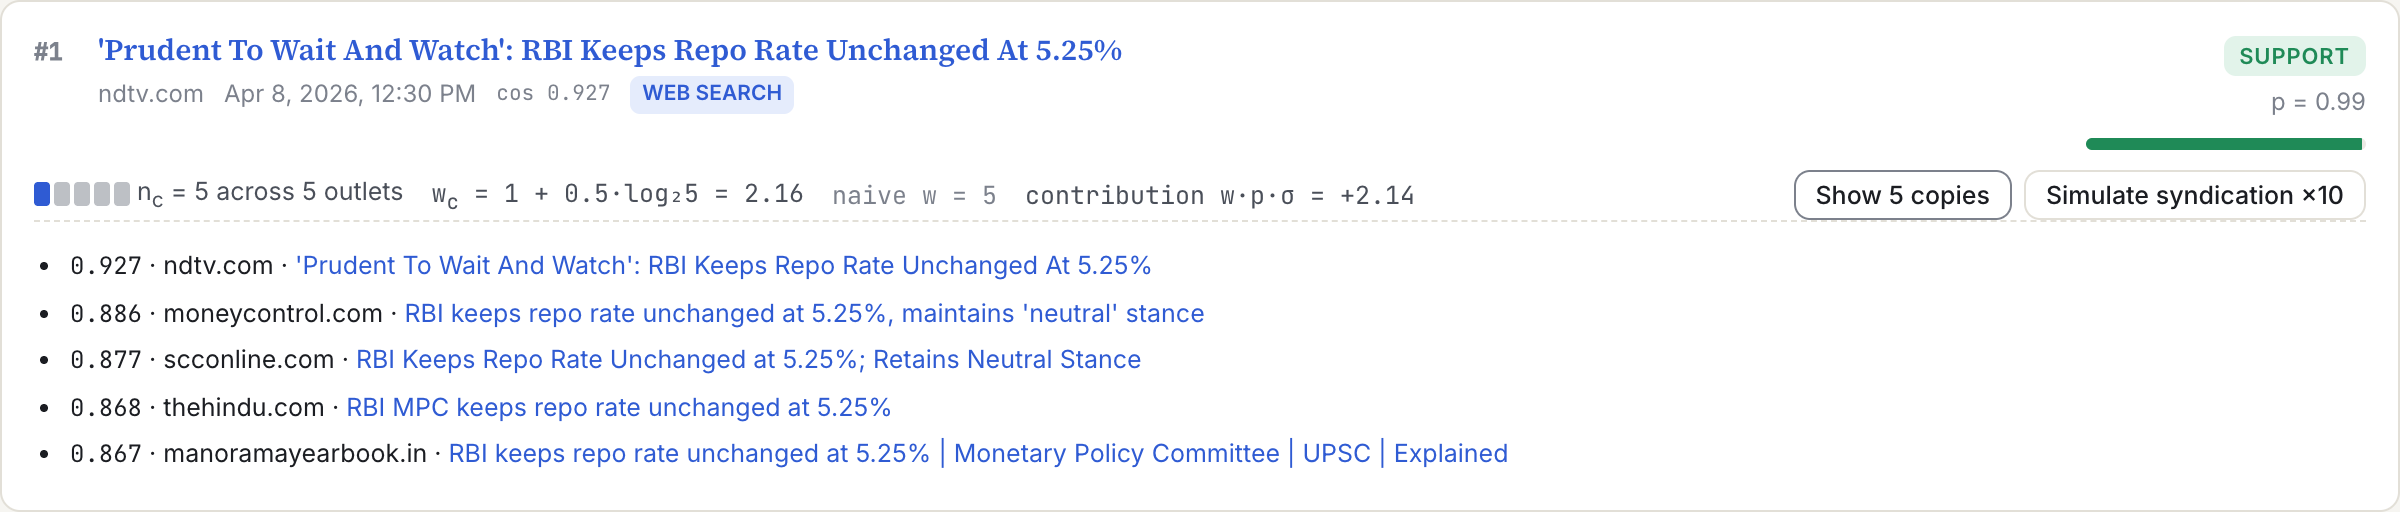
\includegraphics[width=0.94\textwidth]{ui_evidence.png}\\[-1pt]
{\footnotesize (a) Evidence card: one cluster of five articles from five outlets (the top one fetched by web search); weight
$w_c=2.16$ instead of a naive 5.}\\[5pt]
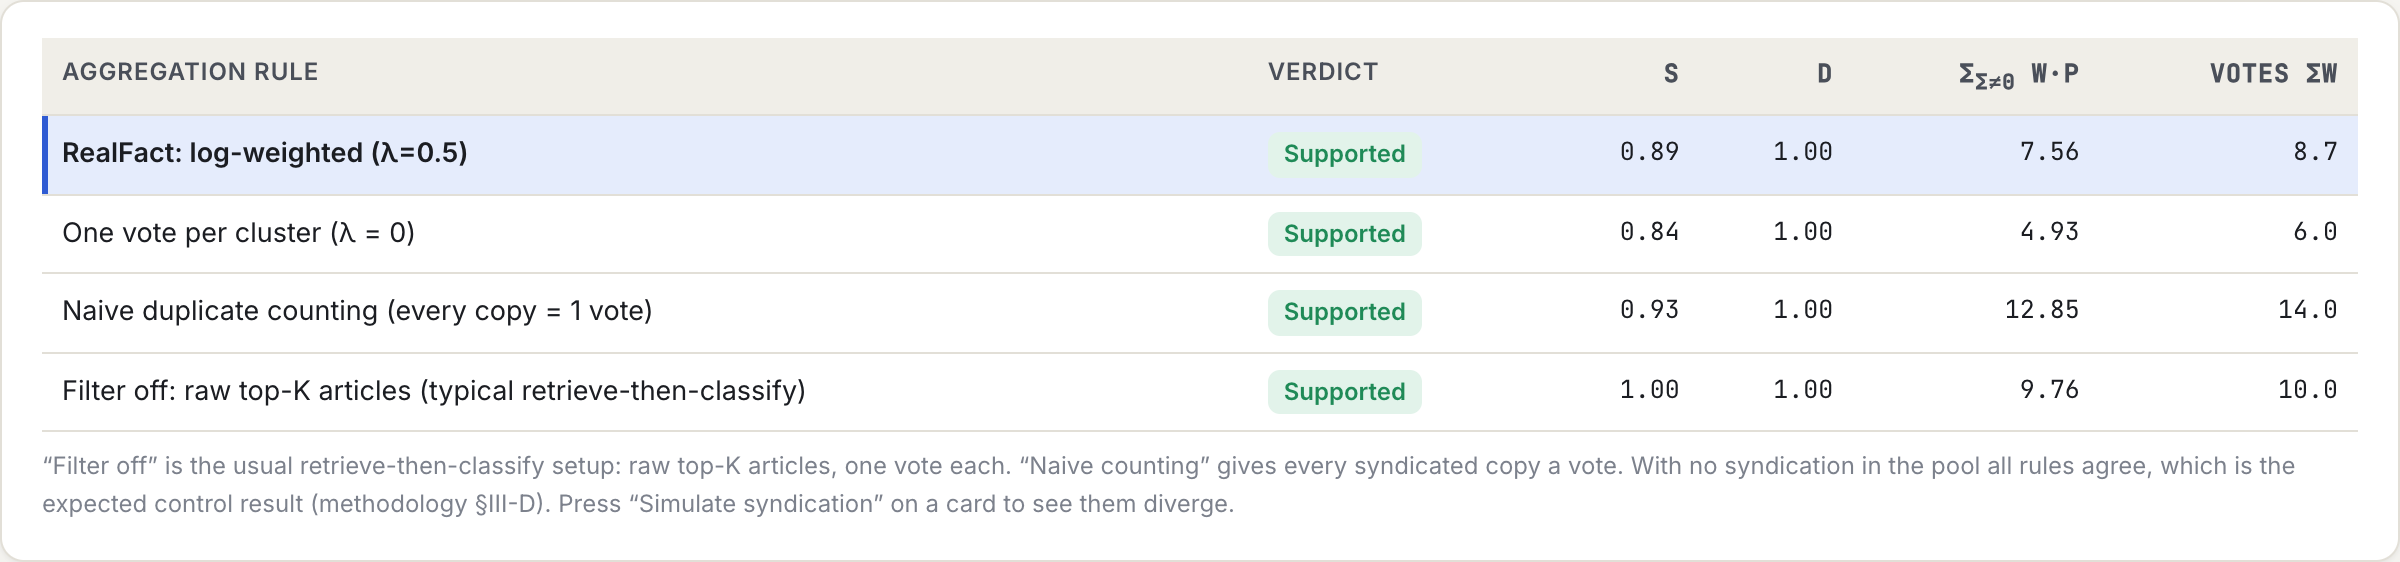
\includegraphics[width=0.94\textwidth]{ui_rules.png}\\[-1pt]
{\footnotesize (b) Existing aggregation rules vs.\ RealFact on the same evidence; without syndication all rules agree, the
expected control result.}\\[5pt]

\includegraphics[width=0.94\textwidth]{ui_fever.png}\\[-1pt]
{\footnotesize (c) FEVER demo mode: FEVER's gold label and annotated evidence next to RealFact's answer and the gold page's
retrieval rank.}
\caption{Result views of the Verify tab.}
\label{fig:ui-cards}
\end{figure*}

\begin{figure*}[!t]
\centering
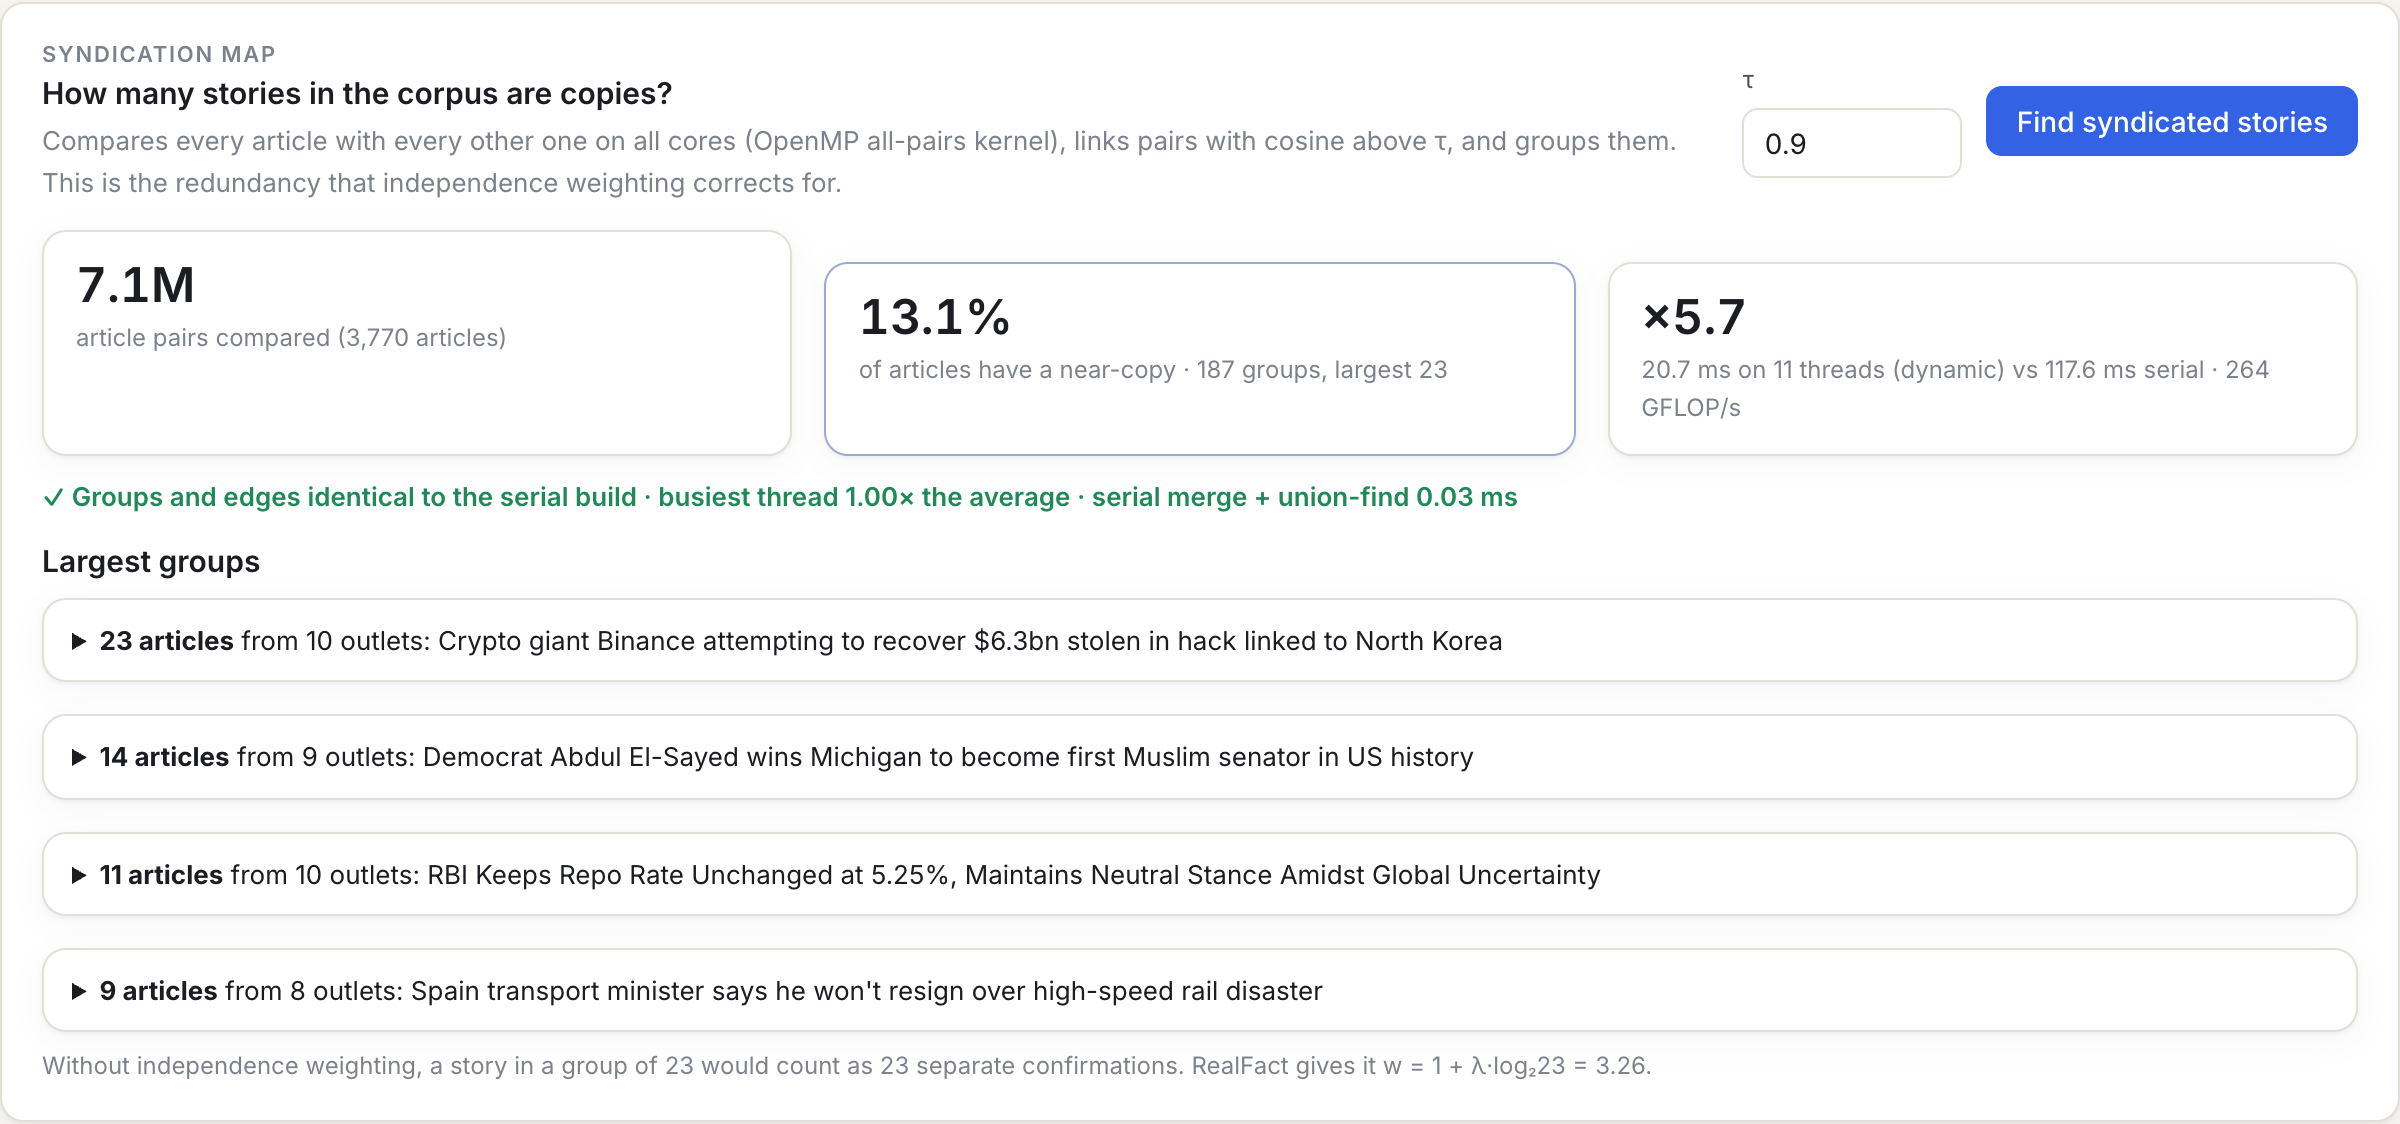
\includegraphics[width=0.86\textwidth]{ui_synmap.png}\\[-1pt]
{\footnotesize (a) Syndication map (Live corpus tab), computed by kernel 2: 7.1M pairs on 11 threads, 13.1\% of articles have
a near-copy, output identical to the serial build.}\\[5pt]
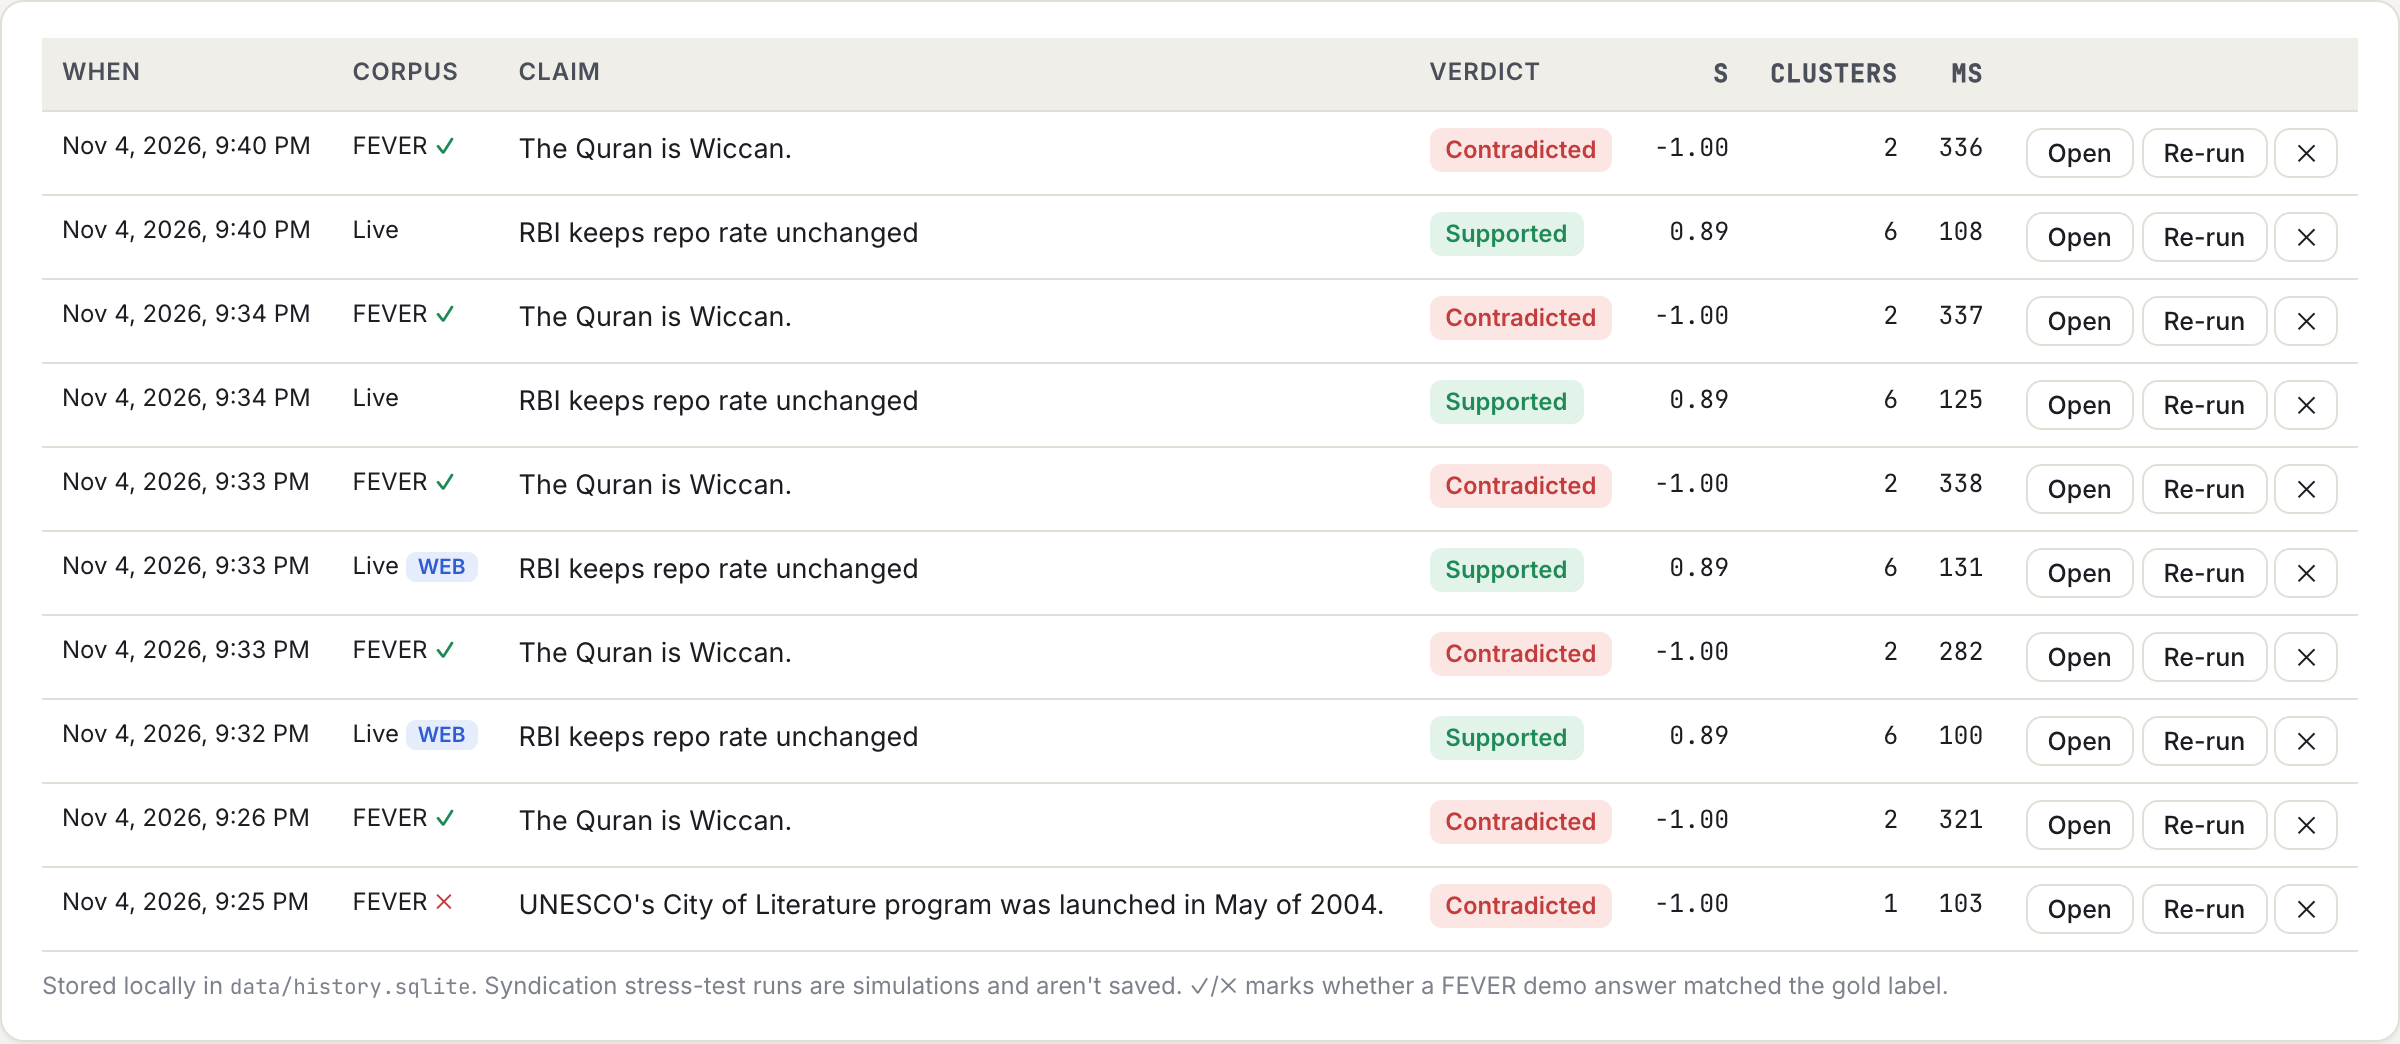
\includegraphics[width=0.86\textwidth]{ui_history.png}\\[-1pt]
{\footnotesize (b) History tab: saved verifications that can be reopened, re-run or deleted; WEB marks checks that used web
search, and \checkmark/$\times$ marks whether a FEVER answer matched the gold label.}
\caption{Corpus-level and history views.}
\label{fig:ui-corpus}
\end{figure*}

% =====================================================================================================
\section{Threats to Validity and Limitations}
\begin{itemize}
  \item \textbf{Syndication vs.\ convergence.} Embedding similarity cannot fully separate syndication from independent
  outlets reporting the same fact, so the filter's effect is an upper bound.
  \item \textbf{No labelled live data.} Live-news accuracy cannot be measured: no labelled dataset matches current news.
  LIAR measures coverage; FEVER is a curated, lead-only subset.
  \item \textbf{NLI behaviour.} The relevance floor and relative cutoff are tuned thresholds; topically similar
  articles about different entities can still be labelled CONTRADICT.
  \item \textbf{Heterogeneous cores, no pinning.} Results reflect the macOS scheduler's placement across performance
  and efficiency cores and are not directly comparable to pinned results on a homogeneous x86 server.
  \item \textbf{Corpus drift.} The live corpus grows between runs; every benchmark records the size it ran on.
  \item \textbf{Web search terms.} The Google News feed is intended for personal, non-commercial use, which covers this
  academic prototype.
\end{itemize}

% =====================================================================================================
\section{Conclusion and Future Work}
RealFact shows that evidence-based news verification over a live, multi-outlet corpus runs in about 100\,ms per claim
on a laptop CPU, and that counting independent sources rather than copies changes verdicts exactly when syndication
is present and leaves them unchanged otherwise. The three OpenMP kernels illustrate three regimes from the course: a
memory-bound scan whose scaling stops at the bandwidth roof (where an ILP rewrite and multi-query blocking were the
effective levers), a compute-bound triangular all-pairs kernel where the choice of schedule decides load balance
($6.92\times$ dynamic vs.\ $4.98\times$ static), and an inherently sequential algorithm made parallel by block
speculation without changing its output. A 14-check suite kept every optimisation bit-exact against the serial build.

Future work: index the full FEVER dump and FakeNewsNet for accuracy comparable to published baselines; measure on a
pinned, homogeneous multi-socket server; use float16 or int8 embeddings to raise the bandwidth ceiling; a heap-free
top-$M$ so batching pays off at large $M$; and generated justifications grounded in the cited clusters.

% =====================================================================================================
\begin{thebibliography}{99}
\bibitem{guo2022} Z.~Guo, M.~Schlichtkrull, and A.~Vlachos, ``A survey on automated fact-checking,'' \emph{Trans.\
Assoc.\ Comput.\ Linguistics}, vol.~10, pp.~178--206, 2022.
\bibitem{fever} J.~Thorne, A.~Vlachos, C.~Christodoulopoulos, and A.~Mittal, ``FEVER: A large-scale dataset for fact
extraction and VERification,'' in \emph{Proc.\ NAACL-HLT}, 2018, pp.~809--819.
\bibitem{liar} W.~Y.~Wang, ```Liar, liar pants on fire': A new benchmark dataset for fake news detection,'' in
\emph{Proc.\ ACL}, 2017, pp.~422--426.
\bibitem{fakenewsnet} K.~Shu, D.~Mahudeswaran, S.~Wang, D.~Lee, and H.~Liu, ``FakeNewsNet: A data repository with news
content, social context, and spatiotemporal information for studying fake news on social media,'' \emph{Big Data},
vol.~8, no.~3, pp.~171--188, 2020.
\bibitem{hover} Y.~Jiang, S.~Bordia, Z.~Zhong, C.~Dognin, M.~Singh, and M.~Bansal, ``HoVer: A dataset for many-hop fact
extraction and claim verification,'' in \emph{Findings of EMNLP}, 2020, pp.~3441--3460.
\bibitem{bge} S.~Xiao, Z.~Liu, P.~Zhang, and N.~Muennighoff, ``C-Pack: Packaged resources to advance general Chinese
embedding,'' arXiv:2309.07597, 2023.
\bibitem{laurer} M.~Laurer, W.~van Atteveldt, A.~Casas, and K.~Welbers, ``Less annotating, more classifying:
Addressing the data scarcity issue of supervised machine learning with deep transfer learning and BERT-NLI,''
\emph{Political Analysis}, vol.~32, no.~1, pp.~84--100, 2024.
\bibitem{openmp} OpenMP Architecture Review Board, \emph{OpenMP Application Programming Interface, Version 5.2}, 2021.
\bibitem{roofline} S.~Williams, A.~Waterman, and D.~Patterson, ``Roofline: An insightful visual performance model for
multicore architectures,'' \emph{Commun.\ ACM}, vol.~52, no.~4, pp.~65--76, 2009.
\bibitem{amdahl} G.~M.~Amdahl, ``Validity of the single processor approach to achieving large scale computing
capabilities,'' in \emph{Proc.\ AFIPS Spring Joint Computer Conf.}, 1967, pp.~483--485.
\bibitem{gustafson} J.~L.~Gustafson, ``Reevaluating Amdahl's law,'' \emph{Commun.\ ACM}, vol.~31, no.~5, pp.~532--533,
1988.
\bibitem{karpflatt} A.~H.~Karp and H.~P.~Flatt, ``Measuring parallel processor performance,'' \emph{Commun.\ ACM},
vol.~33, no.~5, pp.~539--543, 1990.
\bibitem{tarjan} R.~E.~Tarjan, ``Efficiency of a good but not linear set union algorithm,'' \emph{J.\ ACM}, vol.~22,
no.~2, pp.~215--225, 1975.
\end{thebibliography}

\end{document}
